This chapter discusses the pair of tools developed for simulation and analysis of the John Muir, Santa Fe, and other trails prior to moving to a \gls{crn} environment. We found no other application that readily performed the evaluation required for our work so we developed two applications to aid in our research. The two applications, trail runner and trail viewer, are built on published, open-source tools and were designed with extensibility in mind.  Trail runner is a parallel \gls{ga} trail evaluator that manipulates parameters of the simulations and records the runs to a database. Trail viewer is a web-based application that allows users to filter, browse, and view the results from various types of trail simulations. This framework allowed us to easily sweep across different parameters to locate an ideal configuration for later implementation in a \gls{crn}. In this chapter, we will discuss both tools, some of the advantages of these tools, and their framework.

\section{Trail Runner}
Trail runner is responsible for evaluation of different networks to see performance against navigating the agent through different trails (like the John Muir, Santa Fe, and more). Trail runner also performed evolution of the parameters on the networks with \glspl{ga} working towards the maximum performance possible. We have also published trail runner under an open source license and it is available for download at \url{https://github.com/jmoles/trail-runner}. The application is a command line-based Python tool that uses published tools for evaluation of the \glspl{ann} through evolutions in a \gls{ga}.

The \glspl{ann} in trail runner were modeled with PyBrain, a machine learning library for Python~\cite{Schaul2010-tu}. PyBrain served as the basic model for the different flavors of \glspl{ann}. The evolution of the parameters on the \glspl{ann} is performed with \gls{deap}~\cite{Fortin2012-yv}. \gls{deap} is a powerful toolbox allowing straightforward evaluation of \gls{ga} in Python. One of the primary reasons for the selection of \gls{deap} was the tightly integrated use of a distributed computing framework, \gls{scoop}~\cite{Hold-Geoffroy2014-qf}. \gls{scoop} allowed the distributing of work across multiple servers in the lab cluster for reduced run time. With the use of PyBrain, \gls{deap}, and \gls{scoop}, we then had to build a series of tools to evaluate the different trails and report the results.

The intent of trail runner is to allow evaluation of different \gls{ga} and \gls{ann} parameters to attempt and find an ideal solution prior to implementation in a \gls{crn}. Evaluating the same \gls{ann} in a \gls{crn} (with a tool like \gls{coel}~\cite{Banda2014-qw}) can take a substantially longer amount of time. Performing the same optimization in a \gls{crn} from the beginning would have caused the amount of time to simulate this project to increase dramatically. Later, we will show some examples of the speedup with \gls{scoop} and running the same network in \gls{coel}. Easily sweeping across different parameters in trail runner allowed us to narrow the set of potential parameters to run simulations against.

Running the trail runner application is relatively straightforward after users have configured a database for the application to record results and retrieve available configuration parameters. Trail runner uses PostgreSQL~\cite{The_PostgreSQL_Global_Development_Group1996-qt} and includes a script to create the initial database and populate it with the networks and trails used in this work. A safe set of defaults are specified for many of the \gls{ga} parameters, but they are all customizable by the user using command line flags. A few of the key parameters as an example include the trail ID, population size, maximum moves, network ID, and generations to run for. A full list of the available parameters are available in the application's help (\texttt{--help}).

Trail runner took advantage of these tools for evaluation of the trail task. Testing on the tools was performed by first starting with a smaller trail shown in Figure~\ref{fig:test_trails}. Afterwards, we moved on by testing the larger John Muir trail and got results similar to that of Jefferson's. Section~\ref{sec:tools_testing_results} discusses the results of testing against test trail 1, test trail 2, and the John Muir trail.

\begin{figure}
\centering
\begin{subfigure}[b]{.5\textwidth}
    \centering
    
\includegraphics[width=.4\linewidth]{small_trail_1}
    \caption{Test trail 1}
    \label{fig:test_trail_1}
\end{subfigure}%
\begin{subfigure}[b]{.5\textwidth}
    \centering
    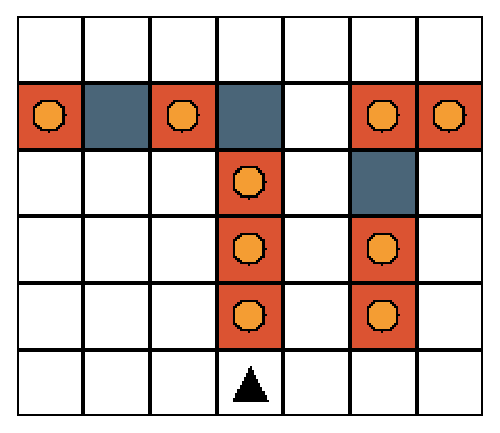
\includegraphics[width=.5\linewidth]{small_trail_2}
    \caption{Test trail 2}
    \label{fig:test_trail_2}
\end{subfigure}
\caption[Two Test Trails]{The two trails used for initial testing of trail runner. They are designed for fast evaluation as well as a small complication (turns, gaps) so that some \gls{ga} optimization is necessary. Test trail 1 is simpler than the test trail 2 on the right.}
\label{fig:test_trails}
\end{figure}

\section{Trail Viewer}
Trail viewer is a Flask~\cite{Ronacher2010-mn} web-based application that allows viewing of results from trail runs over their \gls{ga} evaluation. Diagrams of results are rendered with the help of matplotlib~\cite{Hunter2007-yc} and Plotly~\cite{Plotly2012-po}. The trail diagrams (like the ones in Figure~\ref{fig:test_trails}) used throughout this work are also rendered using trail viewer. At the time of this writing, an instance of trail viewer is operating at \url{http://codeboxide.joshmoles.com}. Figure~\ref{fig:trail_viewer_ss} shows a screen shot of the trail viewer application. Trail viewer is also available under an open source license for download at \url{https://github.com/jmoles/trail-viewer}.

Early versions of trail viewer were a desktop-based \gls{gui}. The application was migrated to a web-based tool for greater compatibility with different operating systems as well as allowing interaction with other web-based tools (like \gls{coel}~\cite{Banda2014-qw} and Plotly~\cite{Plotly2012-po}). Trail viewer also interacts with the same database that trail runner writes results from each run. Trail viewer only consumes information from the database and does not perform any modification. Animation of the agent navigating through the trail is also available in trail viewer. Trail viewer uses JavaScript to render the agent navigating through the trail with a specified trail and moves. The diagrams showing the moves the agent traveled (for example, Figure~\ref{fig:trail1_final_gen}) were captured with the help of this capability.

\begin{figure}
\centering
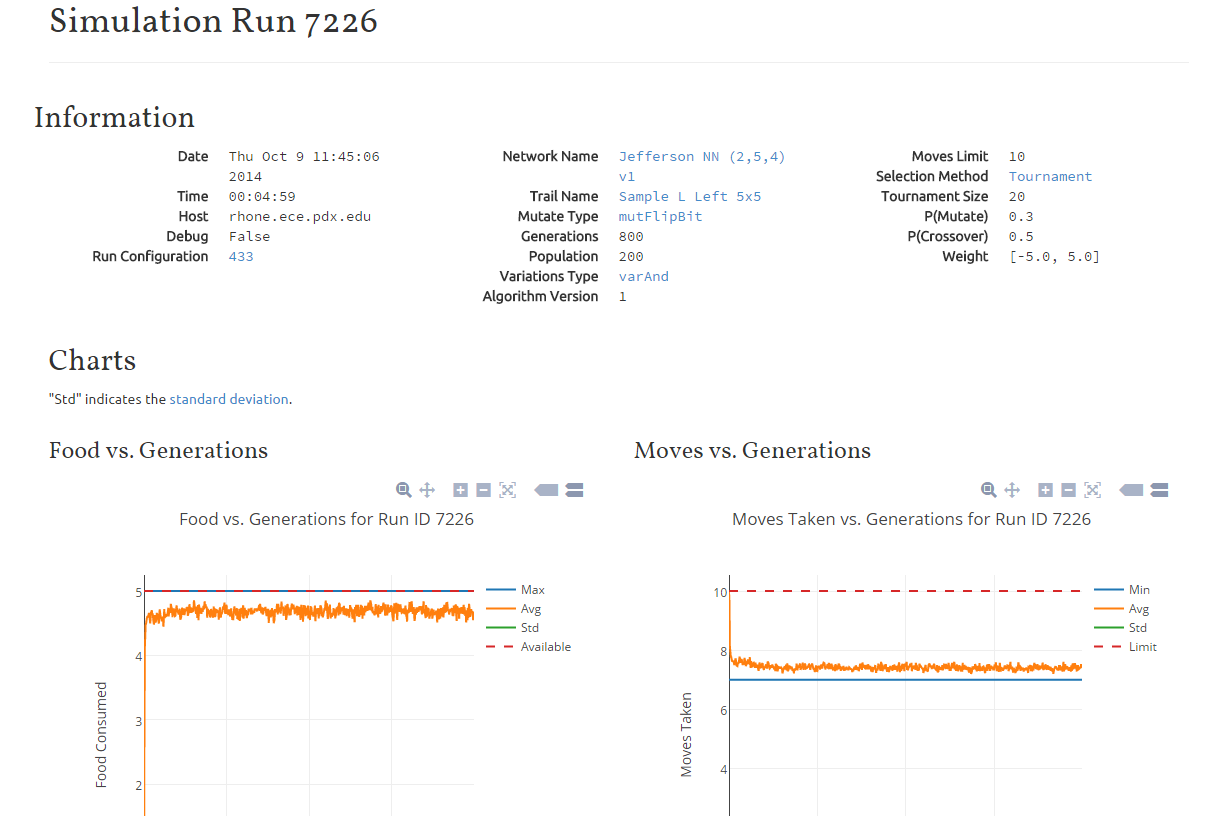
\includegraphics[width=15cm]{trail_viewer_ss}
\caption[Screen Shot of Trail Viewer]{Screen shot of the trail viewer application showing the results of a single simulation run. The information of the trail and simulation configuration is shown at the top with the partial charts of results shown below.}
\label{fig:trail_viewer_ss}
\end{figure}

The pair of these applications provide an environment to evaluate different types of networks and trail problems with numerous sets of parameters and view the results. The integration of PyBrain, \gls{deap}, and \gls{scoop} create a platform that allows others to easily run research similar to that of Jefferson or Koza on the John Muir, Santa Fe, or other trail of choosing. Users can easily add their own databases, networks, or \gls{ga} parameters and generate plots showing a single configuration run, an average of all runs with these parameters, or evaluate a sweep of different parameters, such as delay line length.

In the next chapter, we present the use of trail runner and trail viewer to arrive at the minimal delay line length for implementation in a \gls{crn}.